\section{Descripción de la Empresa o Institución.}

\begin{description}
	\item [Nombre de la Empresa o Institución:] Instituto Nacional de Astrofísica, Óptica y Electrónica (INAOE).
	\item [Dirección:] Calle Enrique Erro No. 1, Santa María. C.P. 72840 Santa María Tonantzintla, Puebla.
	\item [Principal Función de la Institución:] Contribuir como centro público de investigación a la generación, avance y difusión del conocimiento para el desarrollo del país y de la humanidad, por medio de la identificación y solución de problemas científicos y tecnológicos y de la formación de especialistas en las áreas de Astrofísica, Óptica, Electrónica, Ciencias Computacionales y áreas afines.
    \item [Responsable:] Dr. Luis Enrique Sucar Succar.
    \item [Cargo del responsable:] Líder Técnico del Proyecto “CEMIE -Eólico P12”
    \item [Teléfono:] 247 20 44
    \item [Fax:] 247 25 80
    \item [Página Oficial:] http://inaoep.mx/index.php
    \item [Logo:] 
\end{description}

\begin{figure}[!h]
	\centering
	
\includegraphics[width=3cm]{img/inaoe.png}
    \caption{Logotipo del Instituto Nacional de Astrofísica, Óptica y Electrónica (INAOE).}
\end{figure}

\subsection{Historia.}
El Instituto Nacional de Astrofísica, Óptica y Electrónica (INAOE) fue creado por decreto presidencial el 11 de noviembre de 1971 como un organismo descentralizado, de interés público, con personalidad jurídica y patrimonio propio, ubicado en Tonantzintla, Puebla, con los siguientes objetivos:
\begin{itemize}
	\item Preparar investigadores, profesores especializados, expertos y técnicos en astrofísica, óptica y electrónica.
	\item Procurar la solución de problemas científicos y tecnológicos relacionados con las citadas disciplinas.
	\item Orientar sus actividades de investigación y docencia hacia la superación de las condiciones y resolución de los problemas del país.
	\item Con este decreto el INAOE tiene la facultad de impartir cursos y otorgar grados de maestría y doctorado en las diversas disciplinas que en él se desarrollan.
\end{itemize}

EL INAOE es heredero de una gran tradición científica que data de 1942, cuando Luis Enrique Erro fundó el Observatorio Astrofísico Nacional de Tonantzintla. En aquel entonces, Tonantzintla se escogió como el lugar idóneo para la instalación del Observatorio, el cual cumplía con las exigentes normas de calidad como noches despejadas y en cantidad por año, así como altura geográfica y mínima incidencia luminosa de poblaciones cercanas, ya que en la capital de la República no era posible instalar un moderno Observatorio.
\\

Con la Cámara Schmidt de Tonantzintla se inauguró este Observatorio, abriéndose las puertas a la astronomía moderna en México y Latinoamérica. La importancia del Observatorio Astrofísico de Tonantzintla traspasó las fronteras de México, siendo reconocida la labor realizada por astrónomos reconocidos internacionalmente, entre los que figuraron el mismo fundador Luis Enrique Erro; el Dr. Guillermo Haro, el Prof. Luis Rivera Terrazas, el Dr. Luis Munch y el astrónomo Enrique Chavira, entre otros.
\\
 
El INAOE posee una colección de alrededor de 15 mil placas astro-fotográficas obtenidas en la Cámara Schmidt de diversas regiones de la bóveda celeste, principalmente de las constelaciones de Orión, el Toro, Cáncer, Escorpio, Sagitario, Osa Mayor, Osa Mayor, entre otras. Con esta Cámara se hicieron diversos descubrimientos, siendo el principal el de los objetos Herbig-Haro, considerados como los indicadores del inicio de la formación estelar. También se descubrieron estrellas novas y supernovas, galaxias azules e innumerables estrellas ráfaga, así como el cometa Haro-Chavira, descubierto en 1954 en la región del Toro.
\\
  
Erro fue sustituido en la dirección del Observatorio por el doctor Guillermo Haro, bajo cuya dirección se convirtió en uno de los centros más importantes de América Latina por la calidad del trabajo científico que en él se llevaba a cabo. El mismo Haro se dio cuenta de la importancia para el país de la óptica y la electrónica, por lo que en 1971 decidió fundar el INAOE.
\\
 
En 1972 se fundó el Departamento de Óptica, y dos años después inició sus actividades el Departamento de Electrónica. Desde su creación uno de los principales objetivos del INAOE ha sido la preparación de investigadores jóvenes, capaces de identificar y resolver problemas científicos y tecnológicos en astrofísica, óptica, electrónica y áreas afines. En 1972 se iniciaron los estudios de maestría en Óptica y en 1974 los de Electrónica. En 1984 se inició el programa de doctorado en Óptica, y en 1993 los programas de doctorado en Electrónica; así como la maestría y doctorado en Astrofísica. Finalmente, en agosto de 1998 se inició el programa de maestría y doctorado en Ciencias Computacionales.
\\
  
Para lograr que los estudiantes se encuentren en un ambiente de trabajo adecuado y desarrollen al máximo sus capacidades, se exige de ellos una dedicación de tiempo completo. El INAOE por su parte les proporciona áreas de trabajo, laboratorios y equipo de cómputo, así como apoyo para conseguir becas e instituciones nacionales y extranjeras.

\subsection{Misión.}
Contribuir como centro público de investigación a la generación, avance y difusión del conocimiento para el desarrollo del país y de la humanidad, por medio de la identificación y solución de problemas científicos y tecnológicos y de la formación de especialistas en las áreas de Astrofísica, Óptica, Electrónica, Ciencias Computacionales y áreas afines.
 
\subsection{Visión.}
El INAOE será un centro público de investigación con un alto liderazgo a nivel internacional en el ámbito de la investigación científica, el desarrollo tecnológico y la formación de recursos humanos dentro de las áreas de Astrofísica, Óptica, Electrónica, Ciencias Computacionales y áreas afines, comprometido con el desarrollo nacional a través de la promoción de valores sociales de solidaridad, creatividad y alta competitividad.

\subsection{Estructura organizacional.}
El Instituto Nacional de Astrofísica, Óptica y Electrónica cuenta con el organigrama representado en la figura \ref{organigrama}, el cual permite estructurar las diferentes responsabilidades y relaciones dentro del Instituto. 

\begin{figure}[!h]
    \centering
    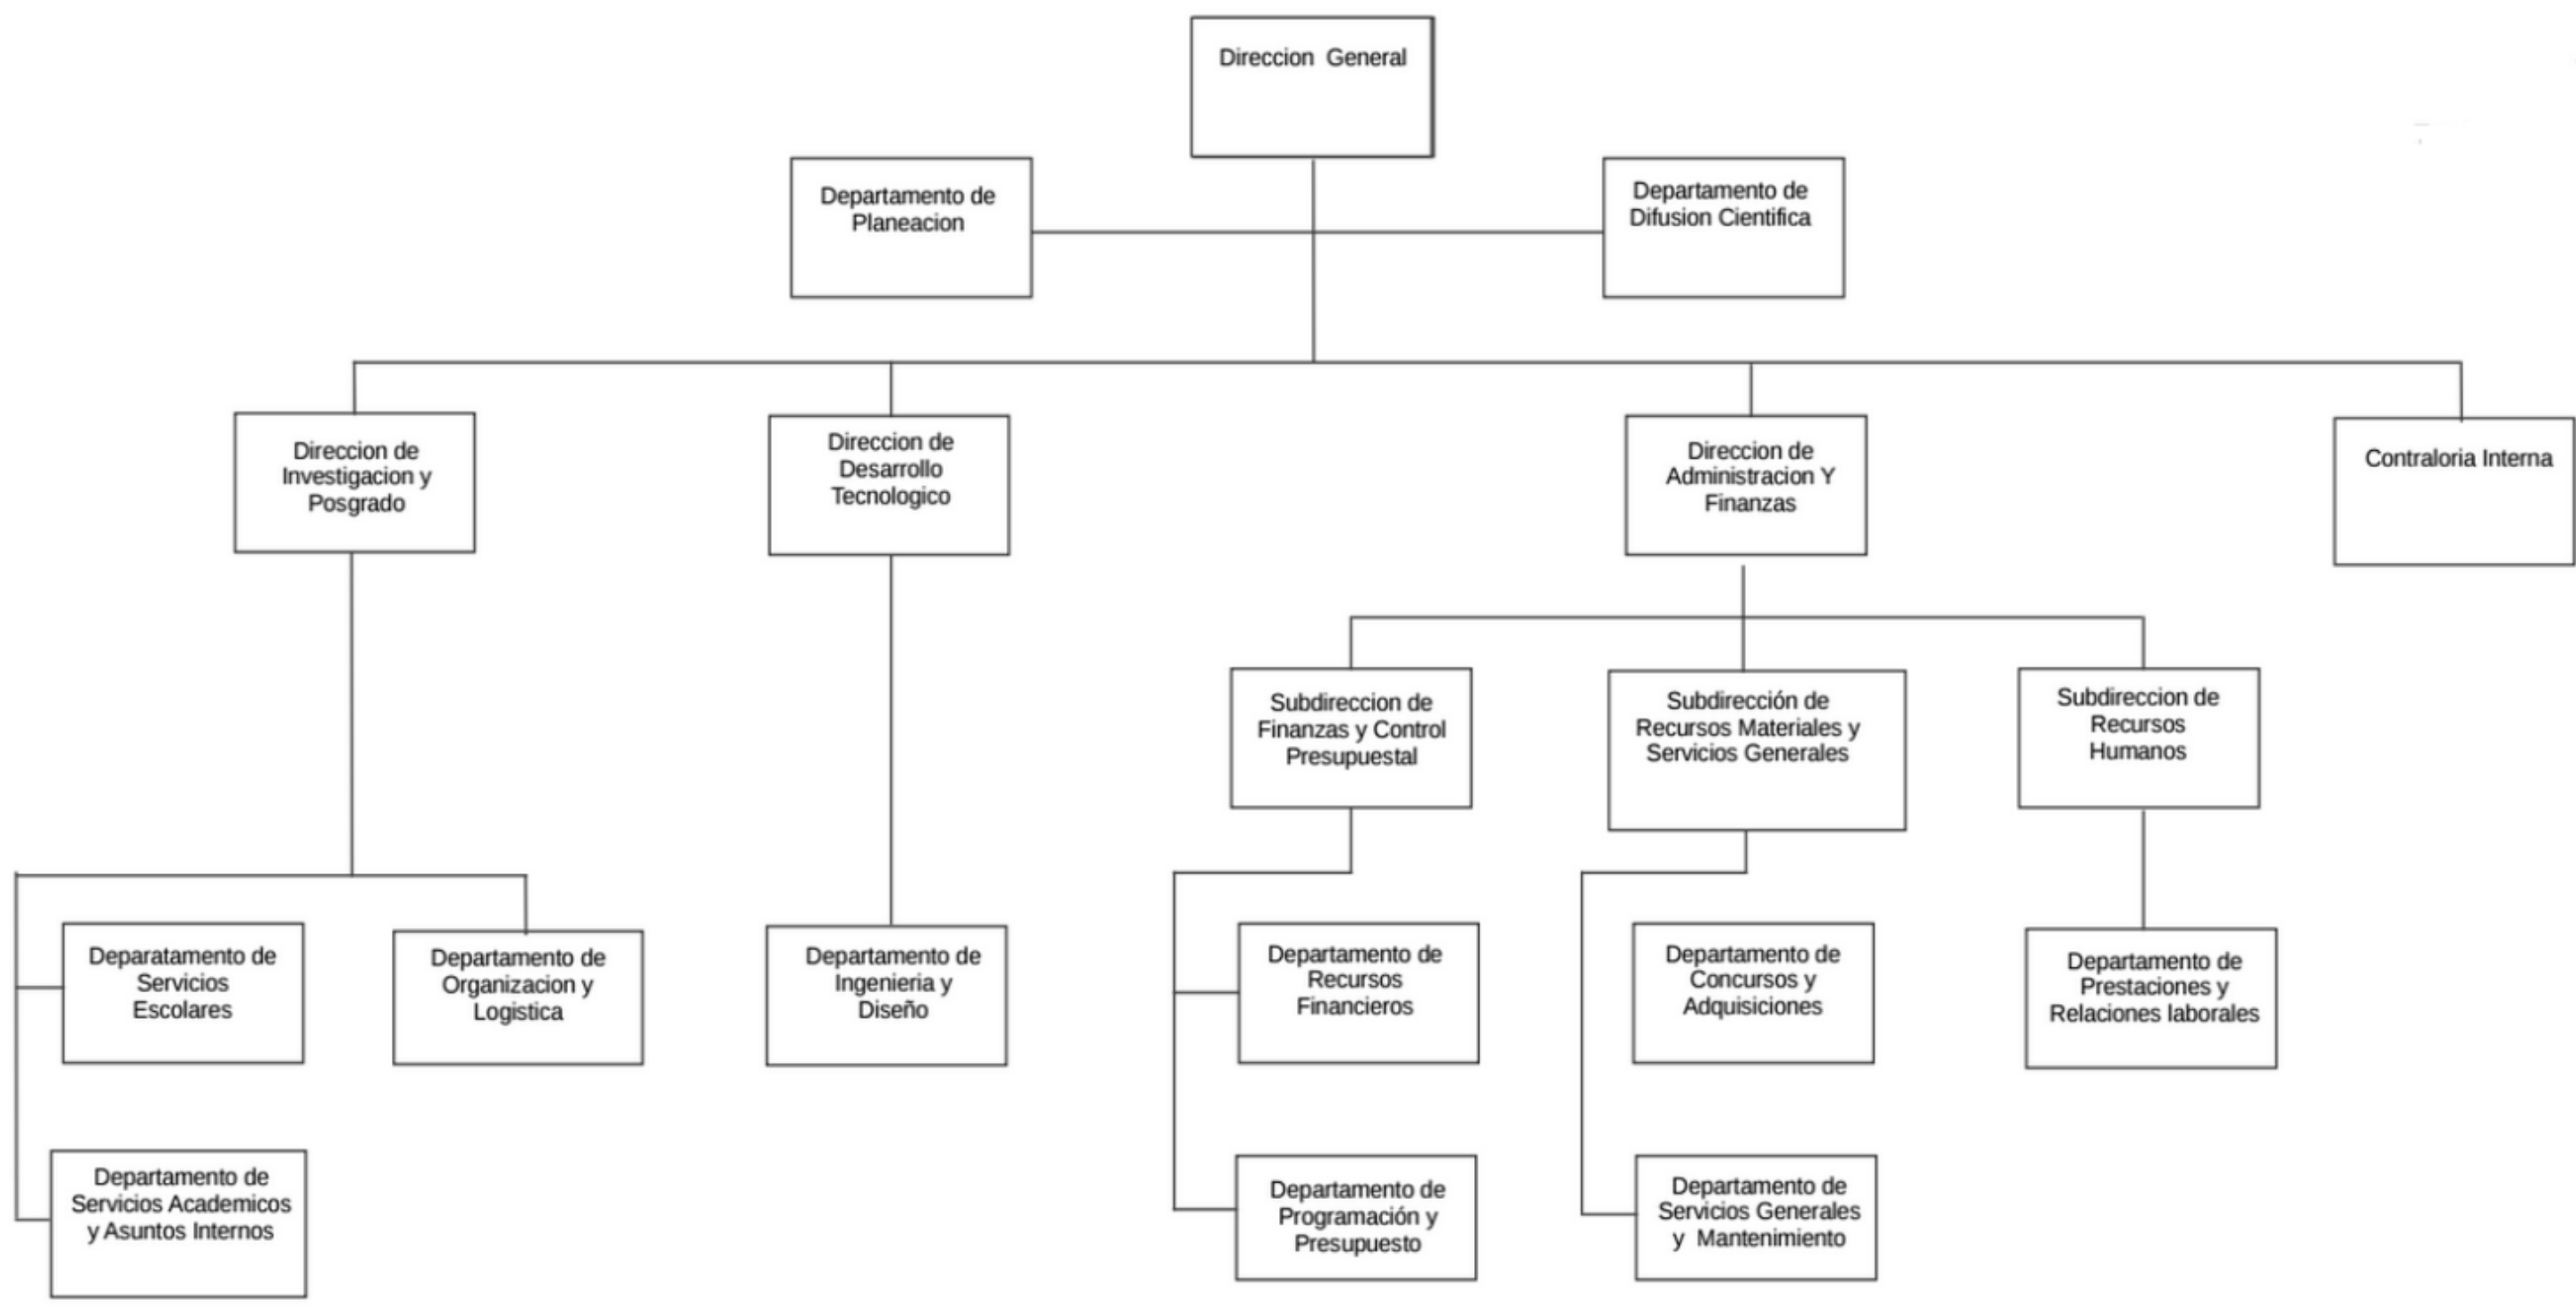
\includegraphics[width=17cm]{img/organigrama.png}
    \caption{Organigrama del INAOE.}
    \label{organigrama}
\end{figure}

\subsection{Área de trabajo.}

Durante el periodo de residencias se cubrió el puesto de programador en el departamento de Coordinación de Ciencias Computacionales en la oficina 8312 en el primer piso, participando en el desarrollo del módulo Agente inteligente de compra venta de energía del proyecto CEMIE-Eólico: Desarrollo de tecnologías basadas en inteligencia artificial y mecatrónica, para integrar un parque de generación de energía eólica una red inteligente.
\\

El equipo de trabajo está conformado por 4 personas:
\begin{itemize}
    \item Líder: Dr. Ansel Y Rodríguez González. 
    \item Programador: David Montero Sifontes.
    \item Programador: Manuel Angel Muñoz Solano.
    \item Programador: Iván Romero García.
\end{itemize}
 
Cada uno cuenta con su propio equipo con las siguientes características:

\begin{itemize}
    \item Memoria: 7.7 GB
    \item Procesador: Intel Core i-4440 CPU, 3.10GHz x 4
    \item Disco Duro: 1 TB
    \item Sistema Operativo Ubuntu 16.04 LTS
\end{itemize} 